\documentclass[tikz,border=6pt]{standalone}
\usepackage{pgfplots}
\pgfplotsset{compat=1.18}
\begin{document}
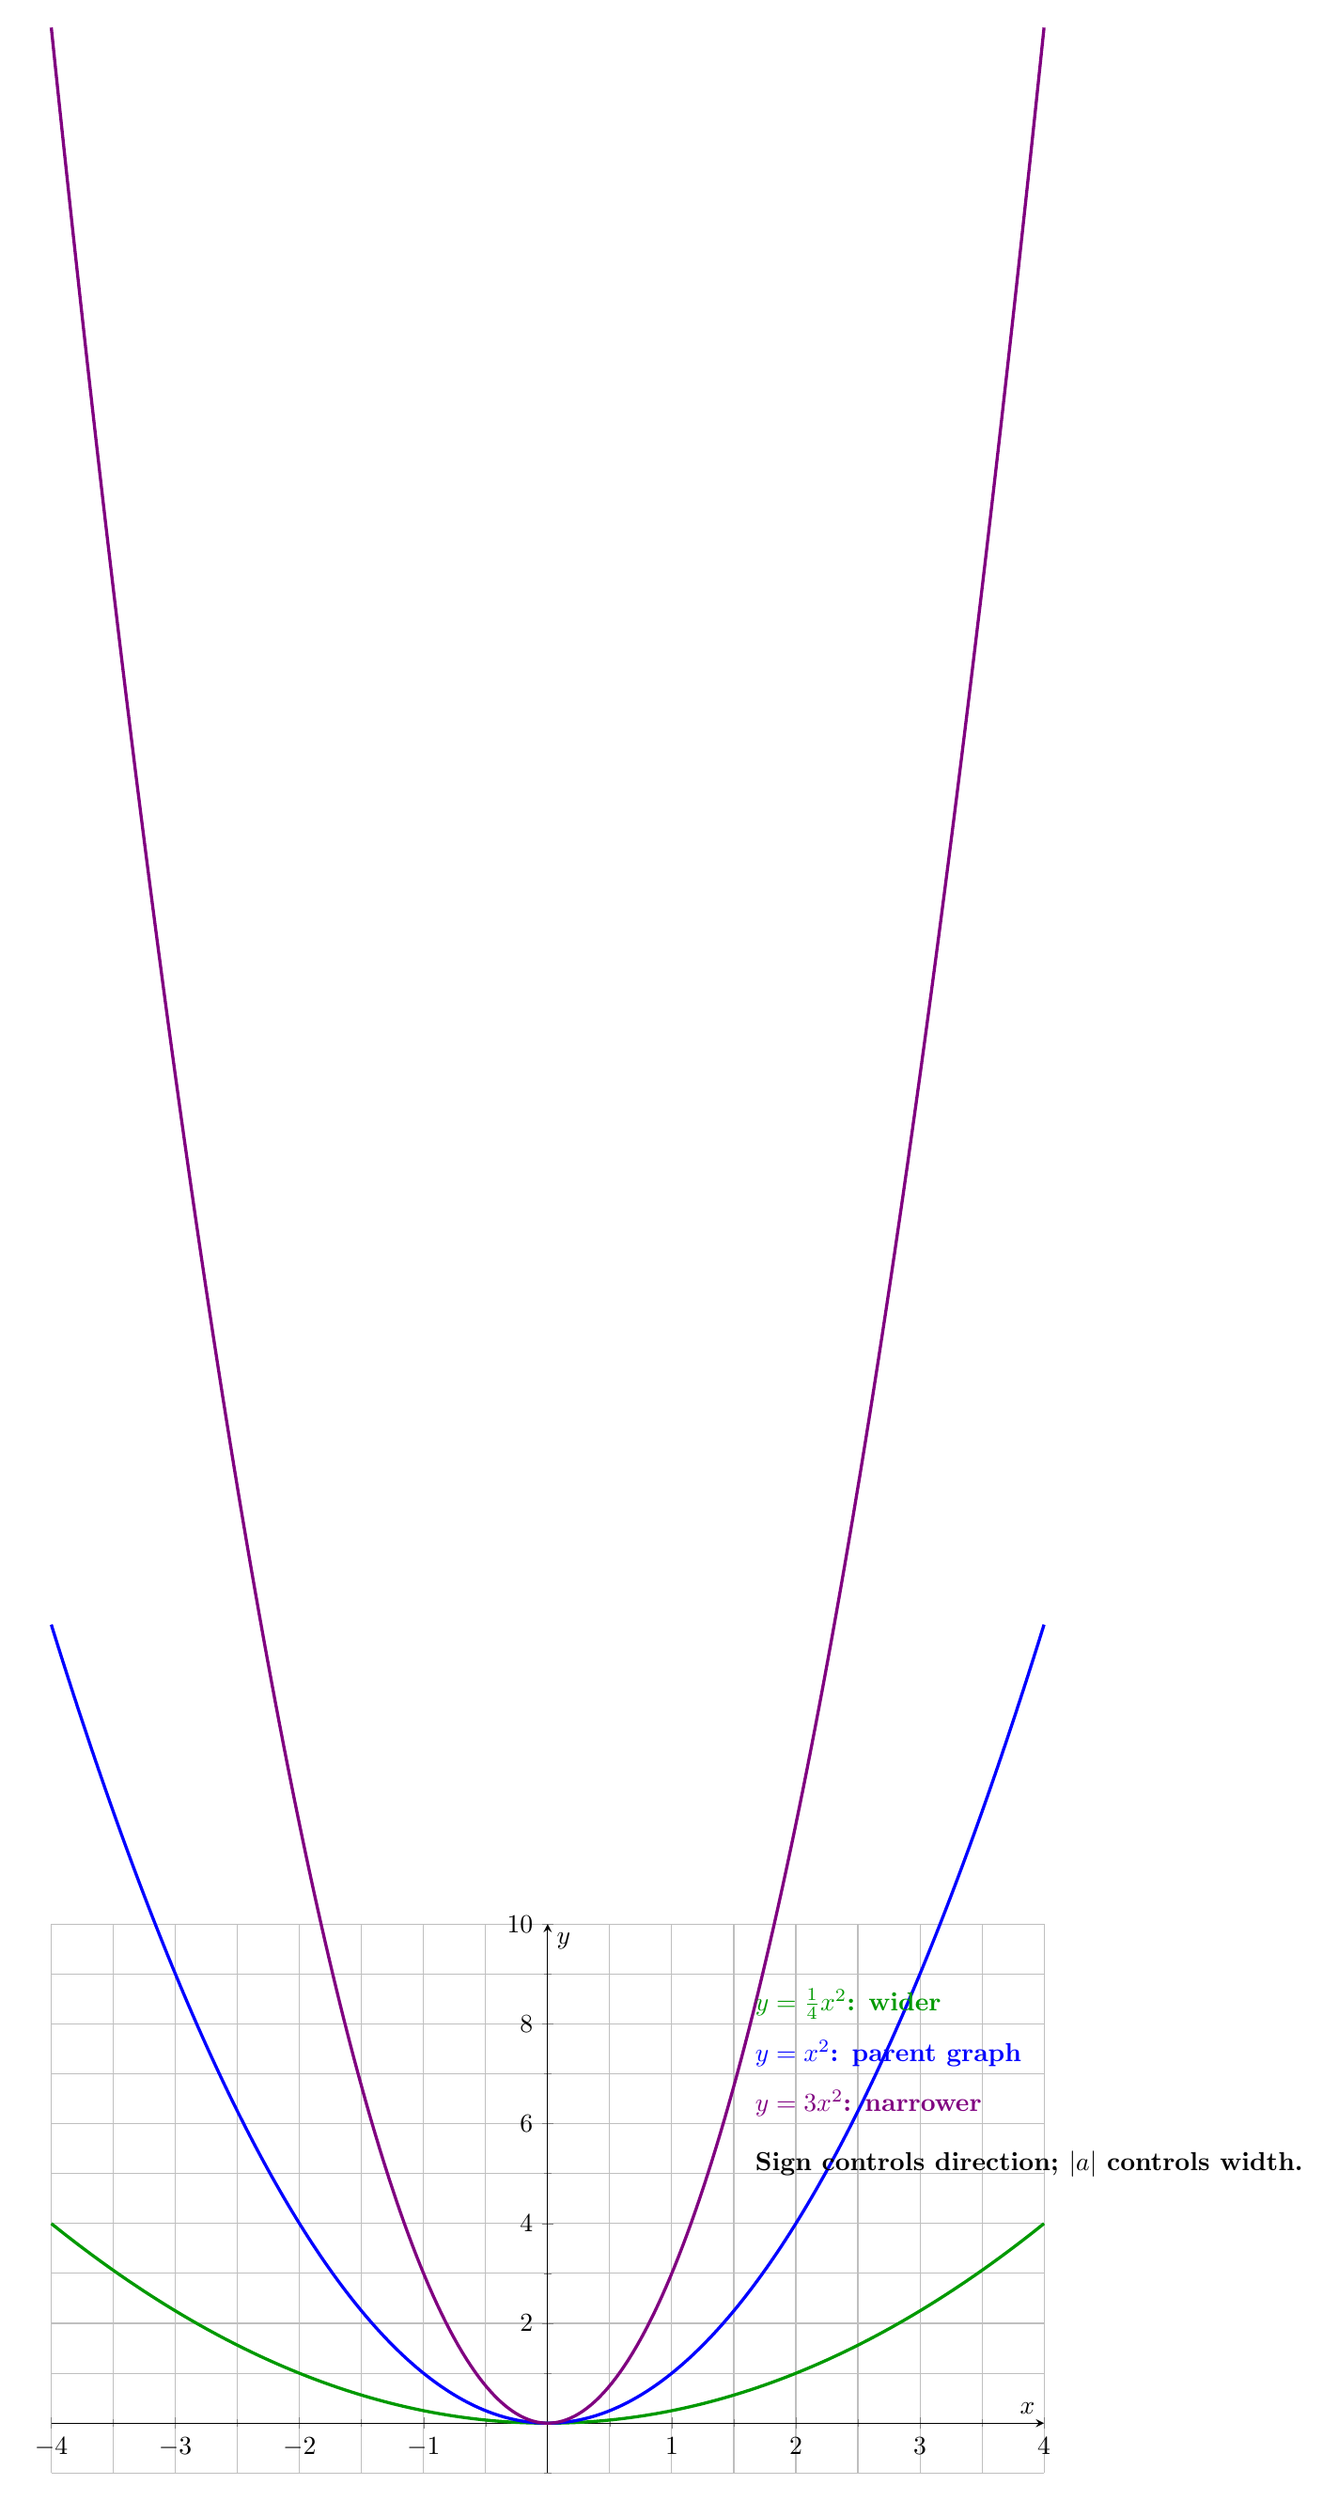
\begin{tikzpicture}
\begin{axis}[
  width=15cm,height=9cm,
  xmin=-4,xmax=4,ymin=-1,ymax=10,
  axis lines=middle,
  xlabel={$x$},ylabel={$y$},
  grid=both,minor tick num=1,
  samples=240,clip=false
]
\addplot[green!60!black,very thick,domain=-4:4]{0.25*x^2};
\addplot[blue,very thick,domain=-4:4]{x^2};
\addplot[violet,very thick,domain=-4:4]{3*x^2};
\node[green!60!black,font=\bfseries,anchor=west] at (axis cs:1.6,8.4) {$y=\frac14x^2$: wider};
\node[blue,font=\bfseries,anchor=west] at (axis cs:1.6,7.4) {$y=x^2$: parent graph};
\node[violet,font=\bfseries,anchor=west] at (axis cs:1.6,6.4) {$y=3x^2$: narrower};
\node[black,font=\bfseries,anchor=west] at (axis cs:1.6,5.2) {Sign controls direction; $|a|$ controls width.};
\end{axis}
\end{tikzpicture}
\end{document}
